% Force plate section, included by main.tex
% =============================================================================
\section{Instrumentation : plateau de force}
\label{sec:plateau}
% =============================================================================

La date de livraison du miroir n'étant pas connue, la partie mesure d'impact est développée sur un support propre au projet : un plateau de force indépendant, qui pourra ensuite être intégré derrière le miroir ou utilisé seul (par exemple pour un miroir de rééducation).

\subsection{Cahier des charges}

Le cadre a été fixé avec M.~Fraisse :
\begin{itemize}
  \item plateau de 1~m $\times$ 1~m ;
  \item capteurs de type FSR (\emph{Force Sensing Resistor}) pour le prototype ;
  \item acquisition sur PC, sans électronique complexe ;
  \item fréquence propre de la structure non calculée, à caractériser lors des essais.
\end{itemize}

L'usage visé est surtout le \emph{shadow boxing} : les utilisateurs touchent la cible plus qu'ils ne frappent à pleine puissance. Le prototype doit fournir l'instant, la position et l'intensité des impacts ; la force absolue en newtons est souhaitable mais pas prioritaire.

\paragraph{Ordres de grandeur.} Sur une plateforme de force verticale échantillonnée à 2~kHz, les crochets arrière de boxeurs de haut niveau atteignent $2\,624 \pm 581$~N (PLOS ONE, 2023). Le dimensionnement retient donc 4\,000~N dans le pire cas, une durée d'impact de 10 à 20~ms et un échantillonnage d'au moins 2~kHz par voie.

\paragraph{Cas défavorable.} Lorsque le coup tombe au droit d'un capteur, ce capteur reprend presque toute la force, quel que soit le nombre de capteurs sous la plaque. Chaque capteur doit donc supporter l'effort total, ou être protégé mécaniquement.

\subsection{Choix du capteur}

\begin{table}[H]
\centering
\begin{tabularx}{\textwidth}{@{}lllX@{}}
\toprule
\textbf{Capteur} & \textbf{Zone sensible} & \textbf{Plage} & \textbf{Évaluation} \\
\midrule
Interlink FSR 406 & 38 $\times$ 38~mm & 0,1 -- 10~N & Plage 400 fois trop faible : détection de contact seulement \\
Tekscan FlexiForce A401 & Ø~25,4~mm & 111~N & Plage étendue non documentée \\
\textbf{Tekscan FlexiForce A201-100} & Ø~9,5~mm & \textbf{445~N}, jusqu'à $\approx$ 4\,400~N & \textbf{Retenu} : plage étendue par réglage du circuit \\
\bottomrule
\end{tabularx}
\caption{Capteurs FSR étudiés.}
\end{table}

Les gammes 4,4~N, 111~N et 445~N de la fiche technique de l'A201 correspondent à trois versions du capteur ; la version 100~lb (445~N) a été retenue. Le constructeur indique que la gamme se déplace avec le circuit : une tension d'excitation et une résistance de contre-réaction plus faibles l'étendent jusqu'à environ 1\,000~lb.

\paragraph{Performances annoncées.} La fiche technique donne les performances typiques suivantes, mesurées avec le montage à amplificateur opérationnel recommandé par le constructeur :

\begin{table}[H]
\centering
\small
\begin{tabularx}{\textwidth}{@{}l>{\raggedright\arraybackslash}p{0.34\textwidth}>{\raggedright\arraybackslash}X@{}}
\toprule
\textbf{Paramètre} & \textbf{Valeur} & \textbf{Conséquence pour le plateau} \\
\midrule
Linéarité & < ±3~\% (droite de 0 à 50~\% de la charge) & Pleine échelle réglée au-dessus des coups attendus \\
Répétabilité & < ±2,5~\% de la pleine échelle & Valable sur capteur conditionné : cycles de charge avant l'étalonnage \\
Hystérésis & < 4,5~\% de la pleine échelle & Principale source d'erreur : la décharge ne suit pas la montée \\
Dérive & < 5~\% par décade de temps, sous 111~N constants & La précharge dérive lentement : tare au démarrage et avant chaque série \\
Temps de réponse & < 5~µs & Négligeable devant un coup de 10 à 20~ms \\
Température & 0,36~\%/°C ; fonctionnement de -40 à 60~°C & Étalonner et mesurer à la même température \\
Durée de vie & $\geq$ 3 millions d'appuis à 22~N & Usure plus rapide sous de fortes charges : capteurs de rechange et ré-étalonnage \\
\bottomrule
\end{tabularx}
\caption{Performances typiques du FlexiForce A201 (fiche technique Tekscan) et conséquences.}
\label{tab:perf}
\end{table}

Une fois les capteurs étalonnés, la précision attendue est de l'ordre de 5 à 10~\% de la pleine échelle par capteur, ce qui suffit pour estimer l'intensité d'un coup et localiser l'impact. La fiche confirme aussi plusieurs choix de conception : seules les deux broches extérieures du connecteur sont actives, la zone sensible mesure 9,53~mm de diamètre (le palet de 9~mm reste à l'intérieur), et le constructeur recommande des palets de répartition de charge (en delrin), comme celui du module de coin. En revanche, elle ne donne pas la résistance du capteur en fonction de la force : elle sera mesurée sur les capteurs reçus.

\subsection{Géométrie du plateau}

Une étude de dimensionnement (document séparé) a établi les bornes de la conception :
\begin{itemize}
  \item \textbf{3 capteurs au minimum} : une plaque unique en appui isostatique donne la force totale et le point d'impact par barycentre des efforts ;
  \item \textbf{3 ou 4 capteurs par plaque} : 3 évite tout calage, 4 convient mieux à une plaque carrée mais nécessite un réglage ;
  \item \textbf{plaques de 10~cm au minimum} : en dessous de la taille du contact du gant, la localisation ne s'améliore plus ;
  \item \textbf{limite d'une acquisition sur PC seul} : environ 16 voies avec une carte d'acquisition USB courante, 50 avec un multiplexeur intégré ; au-delà, un microcontrôleur devient nécessaire.
\end{itemize}

La configuration complète envisagée comporte 4 plaques de 50~cm avec 4 capteurs chacune (16 voies).

\subsection{Prototype retenu}

Le prototype est la première étape de cette configuration : \textbf{une plaque sur 4 FlexiForce A201 placés aux coins}. Les capteurs, le circuit et le logiciel sont identiques à ceux de la version 16 voies, qui ne demandera donc aucune reprise de conception.

L'acquisition se fait avec une carte \textbf{NUCLEO-F072RB} (ADC 12~bits, 1~MS/s), reliée au PC par le port série virtuel du ST-LINK. Ce choix, validé avec M.~Fraisse, permettra en outre de générer le signal de déclenchement des caméras avec la même horloge que les capteurs, ce qui facilitera la synchronisation (livrable~3).

Matériel commandé le 9/11/2026 : 6 FlexiForce A201-100 (DigiKey) et 2 amplificateurs MCP6004 (Farnell). Le reste (plaques, visserie, impression 3D, composants passifs) est disponible sur place.

\subsection{Mécanique d'un module de coin}
\label{sec:meca}

Le plateau est constitué de deux plaques : une \textbf{plaque de base} fixe et une \textbf{plaque de frappe}, recouverte de mousse, qui reçoit les coups. Elles sont reliées par quatre \textbf{modules de coin}, un par capteur (figure~\ref{fig:coupe}). Les pièces sont modélisées sous OpenSCAD (\code{hardware/3d/}) et imprimées en 3D.

\begin{figure}[H]
\centering
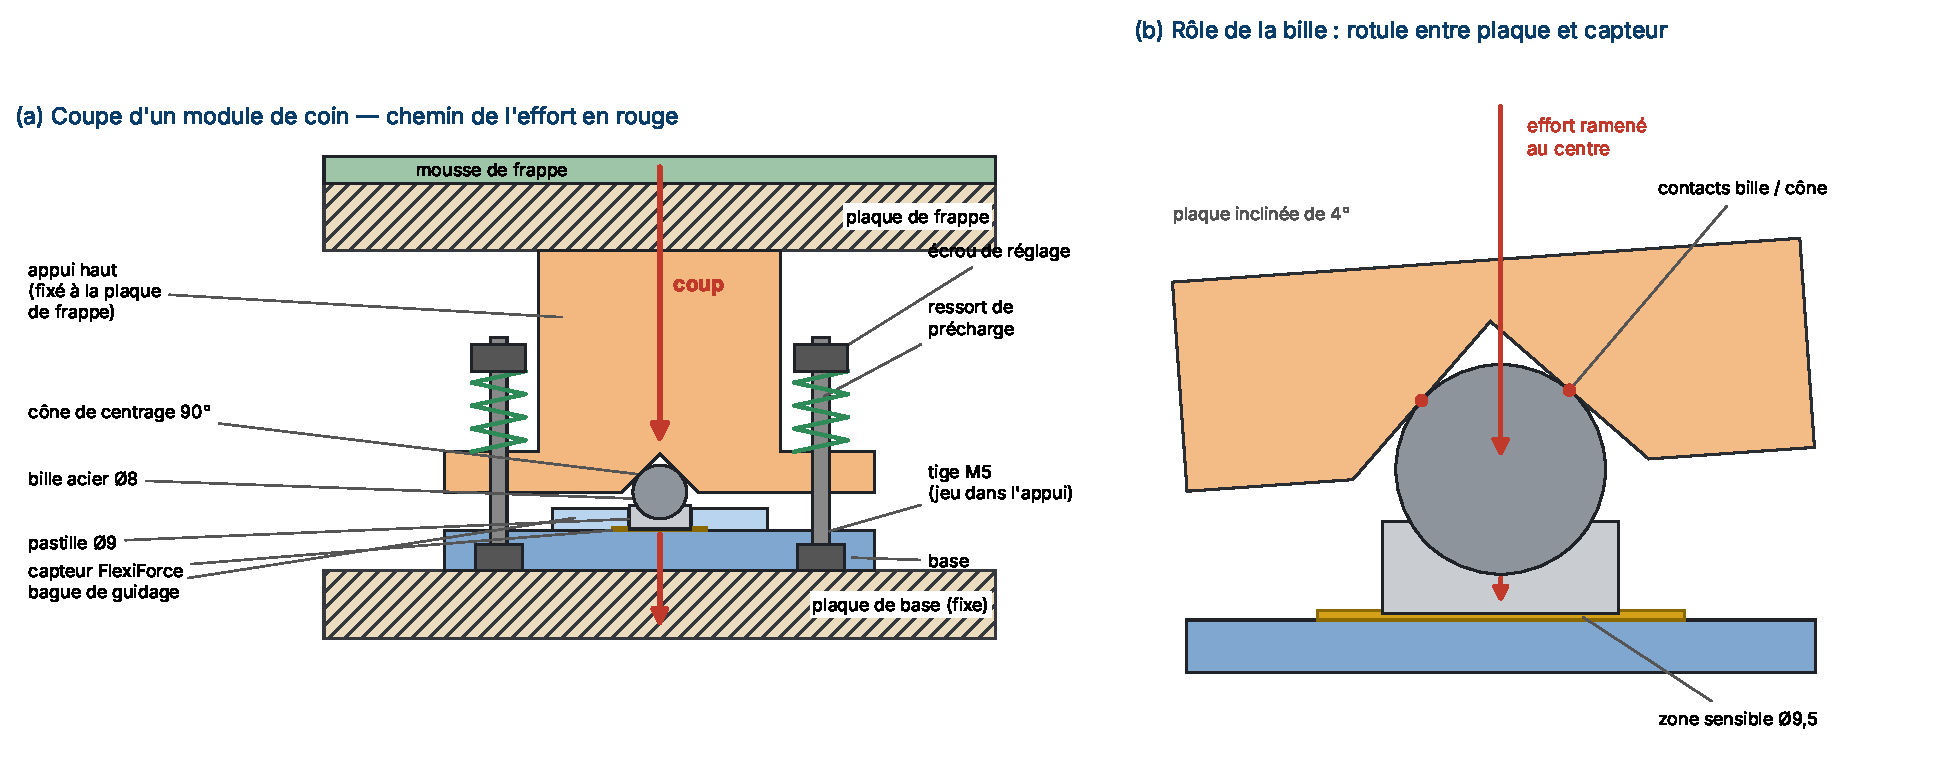
\includegraphics[width=\textwidth]{figures/module_coin_coupe.pdf}
\caption{Module de coin. (a) Coupe et chemin de l'effort. (b) La bille joue le rôle de rotule : même si la plaque s'incline, l'effort arrive au centre du capteur.}
\label{fig:coupe}
\end{figure}

\paragraph{Chemin de l'effort.} Le coup appliqué sur la plaque de frappe est transmis à l'\textbf{appui haut}, vissé sous cette plaque. L'appui porte un \textbf{cône de centrage} à 90° qui repose sur une \textbf{bille en acier} de Ø~8~mm. La bille est logée dans la coupelle d'une \textbf{pastille} de Ø~9~mm, posée sur la zone sensible du capteur (Ø~9,5~mm). Le capteur repose sur la \textbf{base}, vissée sur la plaque de base. Une \textbf{bague de guidage} centre la pastille sur la zone sensible et laisse sortir la queue du capteur. Tout l'effort traverse ainsi le capteur, et rien d'autre.

\paragraph{Rôle de la bille.} Le FlexiForce ne mesure correctement que si l'effort est réparti sur sa zone sensible et appliqué perpendiculairement. Or un coup décentré fait légèrement basculer la plaque de frappe. Avec un appui plat, l'effort se reporterait alors sur un bord de la pastille, qui pincerait le capteur et fausserait la mesure. La bille joue le rôle d'une \textbf{rotule} :
\begin{itemize}
  \item le contact entre le cône et la bille se fait sur un cercle, et l'effort résultant passe toujours par le centre de la bille, quelle que soit l'inclinaison de l'appui ;
  \item la bille ne transmet aucun moment : la pastille reste à plat et charge le capteur uniformément ;
  \item le cône recentre la bille, donc la plaque, à chaque appui : aucun guidage latéral supplémentaire n'est nécessaire.
\end{itemize}
C'est le principe des appuis des plateformes de force et des balances de précision. La pastille est légèrement plus petite que la zone sensible, comme le recommande Tekscan, pour que tout l'effort passe dans la partie active du capteur.

\paragraph{Précharge.} Chaque module porte deux tiges filetées M5, fixées dans la base par des écrous prisonniers. Elles traversent l'appui haut \textbf{avec du jeu} ; au-dessus, un ressort et un écrou appuient l'appui haut sur la bille. Le serrage des écrous :
\begin{itemize}
  \item met l'empilement en contact et maintient la plaque de frappe, y compris en position verticale ;
  \item permet d'équilibrer les quatre coins : avec quatre appuis, une plaque rigide est hyperstatique et l'un des capteurs pourrait ne plus porter.
\end{itemize}
Les ressorts sont beaucoup plus souples que le capteur : lors d'un coup, ils ne reprennent qu'une part négligeable de l'effort, qui passe par le capteur et non par les tiges. La précharge constante est retirée par la tare au démarrage.

\paragraph{Réalisation.} La base, la bague et l'appui haut s'impriment sans support (l'appui haut est imprimé oreilles sur le plateau, le cône ouvert vers le bas avec des pentes à 45°). Le PLA fluant sous charge permanente, la pastille sera remplacée par une pièce en acier ou en résine pour les mesures. Un banc d'essai de 300~mm (\code{test\_rig.scad}) assemble quatre modules et génère les gabarits de perçage des plaques à l'échelle 1:1 ; le même fichier produit le plateau de 1~m.

\subsection{Conditionnement des capteurs}

\begin{figure}[H]
\centering
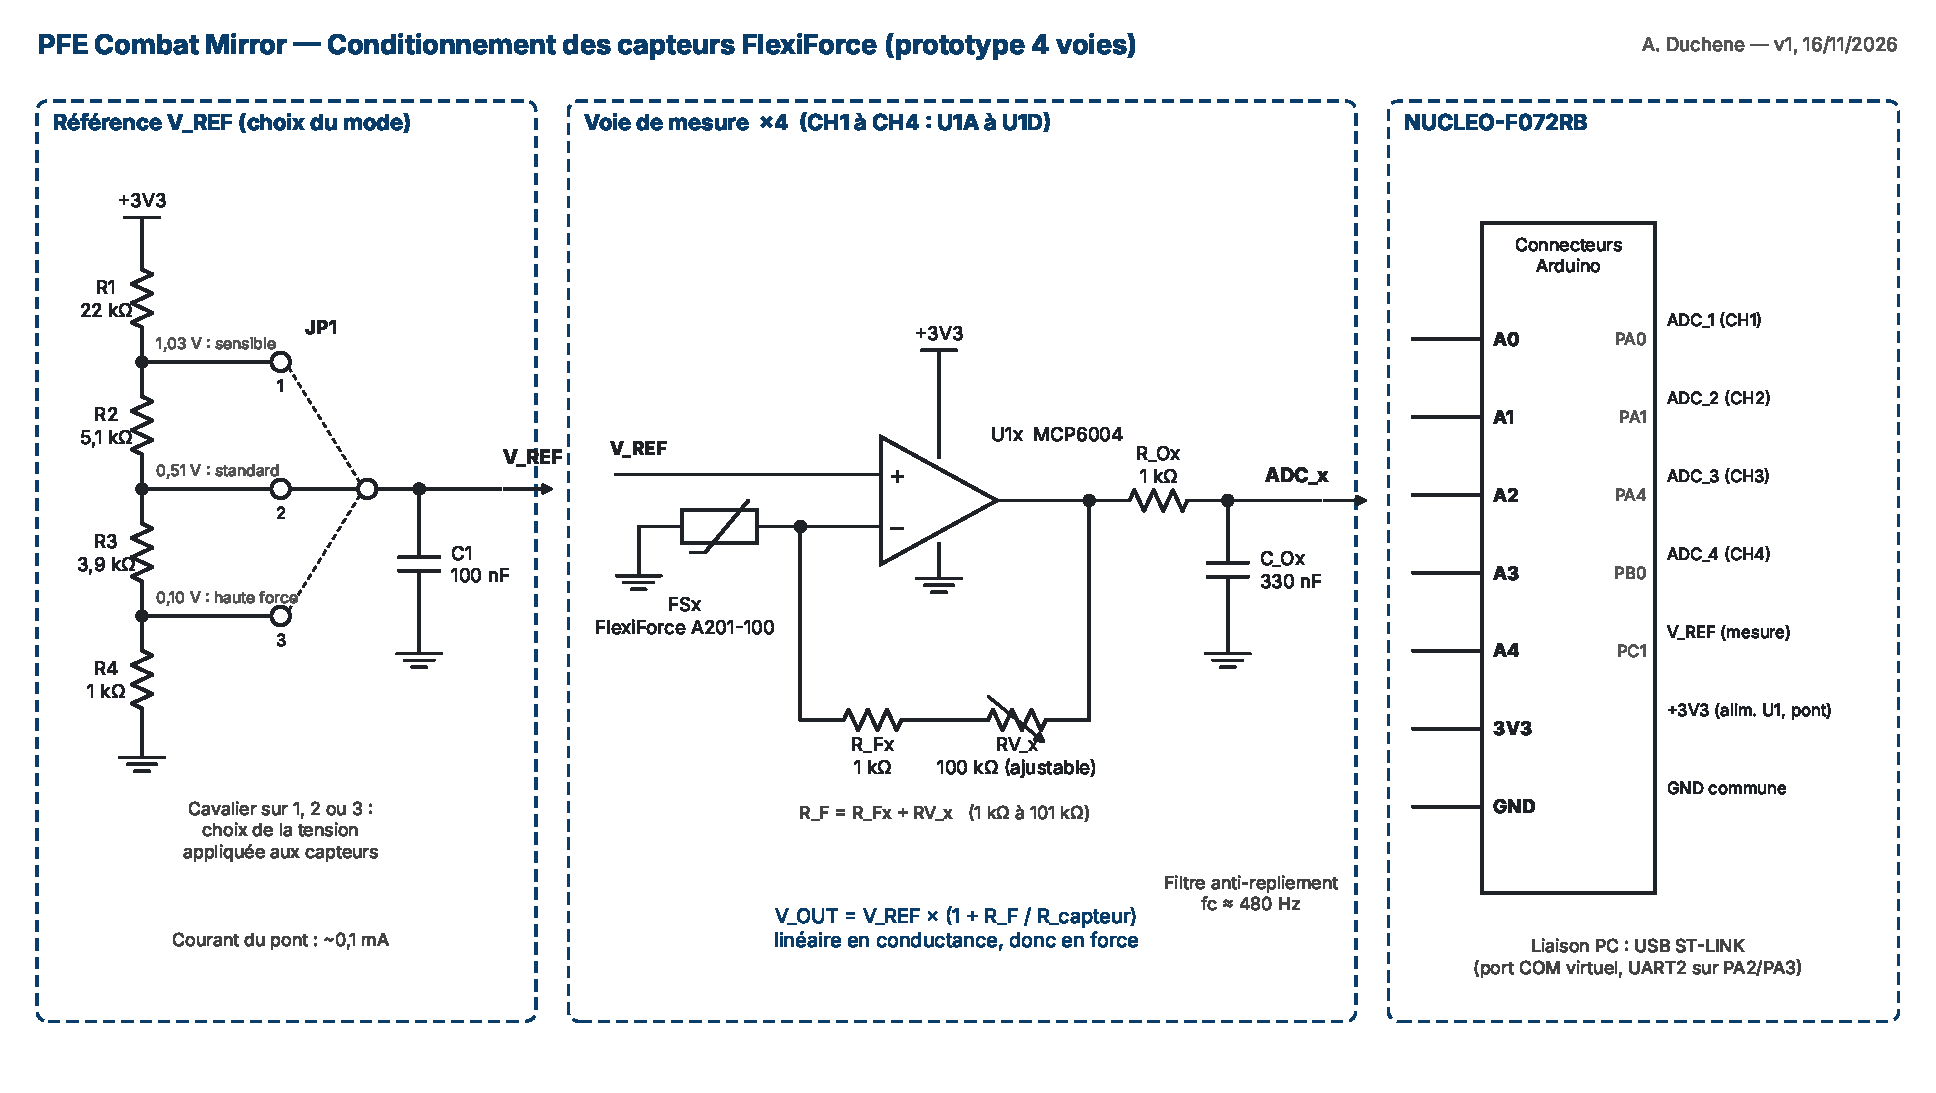
\includegraphics[width=\textwidth]{figures/schema_conditionnement.pdf}
\caption{Schéma de principe du conditionnement (une voie représentée, quatre voies identiques).}
\label{fig:schema}
\end{figure}

Chaque FlexiForce est monté dans un amplificateur non inverseur (figure~\ref{fig:schema}) : le capteur relie l'entrée inverseuse à la masse, la résistance $R_F$ relie la sortie à cette entrée, et l'entrée non inverseuse reçoit la tension de référence $V_{REF}$. On obtient
\begin{equation}
V_{OUT} = V_{REF}\left(1 + \frac{R_F}{R_{capteur}}\right).
\end{equation}
La conductance du FlexiForce étant proportionnelle à la force, la sortie est \textbf{linéaire en force}, avec un décalage égal à $V_{REF}$ à vide. Le capteur est soumis à la tension $V_{REF}$, qui joue le rôle de la tension d'excitation du montage de référence Tekscan, ici sans alimentation négative. Le montage fonctionne en 3,3~V, alimenté par la Nucleo ; un seul MCP6004 conditionne les quatre voies.

\paragraph{Modes de mesure.} Un cavalier choisit $V_{REF}$ sur un pont diviseur, et un potentiomètre de 100~k$\Omega$ par voie règle la pleine échelle :

\begin{table}[H]
\centering
\begin{tabular}{@{}cclc@{}}
\toprule
\textbf{Position} & $\boldsymbol{V_{REF}}$ & \textbf{Mode} & $\boldsymbol{R_F / R_{capteur}}$ \textbf{à pleine échelle} \\
\midrule
1 & 1,03~V & Sensible (touches légères) & 1,9 \\
2 & 0,51~V & Standard ($\approx$ 445~N) & 4,9 \\
3 & 0,10~V & Haute force (jusqu'à $\approx$ 4\,400~N) & 28 \\
\bottomrule
\end{tabular}
\caption{Modes de mesure, pour une pleine échelle de 3,0~V.}
\end{table}

Un filtre RC (1~k$\Omega$, 330~nF, coupure à 480~Hz) précède chaque entrée de l'ADC pour limiter le repliement à 2~kHz d'échantillonnage. Les sorties sont reliées aux entrées A0 à A3 de la Nucleo ; $V_{REF}$ est aussi mesurée (A4) pour que le logiciel connaisse le mode actif et le décalage à vide.

\subsection{Simulation}

Le circuit est simulé sous ngspice (\code{hardware/simulation/}), le FlexiForce étant modélisé par une conductance commandée. Trois analyses vérifient la linéarité et la saturation (balayage DC), la bande passante de la chaîne (analyse AC) et la réponse à un impact de 15~ms (transitoire).

Le tableau~\ref{tab:simu} donne les valeurs attendues en mode standard, pour une résistance du capteur de 10~k$\Omega$ à pleine charge (hypothèse, à remplacer par la valeur mesurée).

\begin{table}[H]
\centering
\begin{tabular}{@{}lcc@{}}
\toprule
\textbf{Grandeur} & \textbf{Calcul} & \textbf{Simulation} \\
\midrule
Tension à vide & 0,505~V & 0,505~V \\
Pleine échelle & 3,00~V & 3,00~V \\
Début de saturation & 108~\% de la pleine échelle & 108~\% \\
Fréquence de coupure & 482~Hz & 481~Hz \\
Pic pour un impact à 80~\% & 2,50~V & 2,50~V (à 12,8~ms) \\
\bottomrule
\end{tabular}
\caption{Résultats de simulation (mode standard, $R_F$ = 49,4~k$\Omega$).}
\label{tab:simu}
\end{table}

Les résultats concordent avec le calcul. Le pic à l'entrée de l'ADC arrive 0,3~ms après celui de l'impact, à cause du filtre, sans perte d'amplitude.

\paragraph{Cas défavorable.} Ces simulations supposent un capteur idéal. Une quatrième simulation (\code{sim\_worstcase.cir}) applique le même impact à trois voies identiques : capteur idéal, capteur avec l'hystérésis de la fiche (4,5~\% de la pleine échelle à la décharge), et capteur cumulant hystérésis et erreur de sensibilité (3~\% de linéarité et 2,5~\% de répétabilité). L'erreur attendue est d'environ 4,5~\% de la pleine échelle dans le deuxième cas et 7~\% dans le troisième, au maximum pendant la décharge. Le pic de force, mesuré en fin de montée, n'est pas touché par l'hystérésis : seule l'erreur de sensibilité (environ 4,4~\%) s'y applique, et l'étalonnage la réduit.

En mode haute force, $R_F$ doit valoir 28 fois la résistance du capteur à 4\,400~N : la plage du potentiomètre (1 à 101~k$\Omega$) convient tant que cette résistance reste inférieure à 3,6~k$\Omega$, ce que le premier essai devra confirmer.

\subsection{Étalonnage prévu}

\begin{enumerate}
  \item \textbf{Capteur seul}, sur un module : quelques cycles de conditionnement à environ 110~\% de la charge d'essai (recommandation Tekscan ; les valeurs de répétabilité et d'hystérésis de la fiche ne valent que pour un capteur conditionné), puis charges connues par paliers ; ajustement d'une droite par capteur, mesure de l'hystérésis et de la dérive.
  \item \textbf{Plateau complet}, posé à plat : masse connue placée sur une grille de points ; vérification que la somme des quatre forces égale le poids et que le barycentre tombe au bon endroit ; correction des gains par moindres carrés.
  \item \textbf{Tare à chaque démarrage} et avant chaque série, pour retirer la précharge et le poids de la plaque, et compenser la dérive sous charge constante.
  \item \textbf{Contrôle périodique} avec une masse connue, les capteurs s'usant plus vite sous de fortes charges que dans l'essai d'endurance du constructeur (22~N).
\end{enumerate}
Un essai de chute (masse connue lâchée d'une hauteur connue) complétera ces mesures statiques par une vérification dynamique.

